\section{Descrição funcional} % (fold)
\label{sec:descricaofuncional}

Texto...

\begin{itemize}
    \item sinal\_exemplo [15:0] - saída 1

\end{itemize}    
     
\par \hspace{2cm}       • 
\par \hspace{2cm}       • 
\par \hspace{2cm}       • 
    
\begin{itemize}           
    \item sinal\_flag - saída 0
\end{itemize}


\subsection{Características e recomendações}

\begin{itemize}
  \item O clock;
\end{itemize}


% Coloque uma figura aqui se precisar...

%\begin{figure}[h]
  %\caption{Diagrama de Tempo.}
  %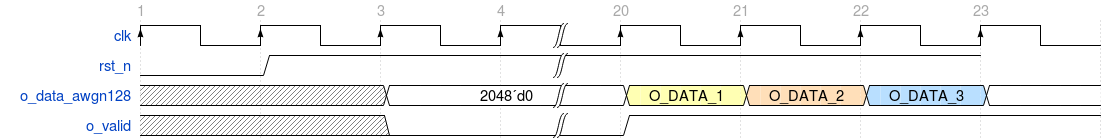
\includegraphics[width=\linewidth]{images/wavedrom.png}
  %\label{fig:top}
%\end{figure}


\subsection{NOME\_SUBSECTION}

Texto...

$$ \Phi(x) = \frac{1}{\sqrt{2\pi}}e^{\frac{-1}{2}x^2} $$

\par A média é dada pela seguinte expresão:

$$ M(x) = \int_{-\infty}^{\infty} x \frac{1}{\sqrt{2\pi}}e^{\frac{-1}{2}x^2} = 0  $$


\begin{itemize}

  \item Texto...
  
\end{itemize}